\documentclass[11pt,a4paper]{report}

\usepackage[T1]{fontenc}
\usepackage[utf8]{inputenc}
\usepackage[english]{babel}
\usepackage{lmodern}
%\usepackage{circuitikz}
\usepackage{color}
\usepackage{wrapfig}
\usepackage{placeins}
\usepackage{subfigure}
\usepackage{tabu}
\usepackage{fullpage}
\usepackage[squaren]{SIunits}
\usepackage{graphicx}
%\usepackage[pdftex]{graphicx}
\usepackage{epstopdf}
\usepackage{epsfig}
\usepackage{hyperref}
\usepackage{tikz}
\usepackage{tikz-qtree}
\usepackage{eurosym}
%\usepackage{chemist}
\usepackage{amsmath}
\usepackage{amssymb}
\usepackage{mathrsfs}
\usepackage{dsfont}% use $\mathds{1}$
\newcommand{\C}{\mathbb{C}}
\newcommand{\N}{\mathbb{N}}
\newcommand{\Z}{\mathbb{Z}}
\newcommand{\R}{\mathbb{R}}
\newcommand{\red}{\textcolor{red}}
\newcommand{\dis}{\displaystyle}
\newcommand{\dr}{\partial}
\newcommand{\txt}{\text}
\newcommand{\td}{\todo[inline]}
\newcommand{\ttt}{\texttt}
\newcommand{\itt}{\textit}

\usepackage{algorithm}
\usepackage{todonotes}
\usepackage[noend]{algpseudocode}

%\newtheorem{theoreme}			     {Théorème}	[chapter]
%\newtheorem{proposition}[theoreme]	 {Proposition}	
%\newtheorem{corollaire}	  [theoreme]	 {Corollaire}	
%\newtheorem{lemme}	      [theoreme]  {Lemme}		
%\newtheorem{definition}	         {Définition}[chapter]
%\theoremstyle{definition}
%\newtheorem{exemple}			     {Exemple}	[chapter]
%\newtheorem{contreexemple}[exemple]{Contre-exemple}
%\newtheorem{probleme}	             {Probl\`eme}[chapter]

\usepackage{listings}
\usepackage{textcomp}
\definecolor{listinggray}{gray}{0.9}
\definecolor{lbcolor}{rgb}{0.9,0.9,0.9}
\lstset{
	backgroundcolor=\color{lbcolor},
	tabsize=4,
	rulecolor=,
	language=matlab,
        basicstyle=\scriptsize,
        upquote=true,
        aboveskip={1.5\baselineskip},
        columns=fixed,
        showstringspaces=false,
        extendedchars=true,
        breaklines=true,
        prebreak = \raisebox{0ex}[0ex][0ex]{\ensuremath{\hookleftarrow}},
        frame=single,
        showtabs=false,
        showspaces=false,
        showstringspaces=false,
        identifierstyle=\ttfamily,
        keywordstyle=\color[rgb]{0,0,1},
        commentstyle=\color[rgb]{0.133,0.545,0.133},
        stringstyle=\color[rgb]{0.627,0.126,0.941},
}

\DeclareMathOperator{\e}{e}

\title{Titre}
\author{Florentin Goyens}
\date{\today}

\begin{document}
\tabulinesep=1.2mm
\begin{center}
\hrule
\begin{tabular}{c}
\\[0.005cm]
\Large{Applied Numerical Methods - Lab 3}\\[0.3cm]
\textsc{Goyens} Florentin  \& \textsc{Weicker} David\\[0.2cm]
$\text{13}^{\text{th}}$ October 2015\\[0.2cm]
\end{tabular}
\hrule
\end{center}


\section*{Stationary heat conduction in 1-D}

In a one dimensional pipe we are interested in the temperature evolution along the z-axis.  We will study the behaviour of the numerical solution based on finite differences.



\subsection*{1) Distretization to a linear system of equations}

The z-axis is first discretized in $N+1$ points spreading from $0$ to $L$. The differential equation for the temperature is the following
$$-\kappa \dfrac{d^{2}T}{dz^{2}} +v\rho C\dfrac{dT}{dz}=Q(z)$$
with $$Q(z)= \left\{ \begin{array}{lll}
0 & if & 0\leq z <a\\
Q_{0}\sin \Big(\dfrac{z-a}{b-a}\pi \Big) & if & a \leq z \leq b\\
0 & if & b\leq z \leq L.\\
\end{array}\right.$$
We assumed that $\kappa$ as a constant value through the pipe.

The boundary conditions are
$$T(0)=T_{0}$$ and $$-\kappa \dfrac{dT}{dz}(L)=k_{v}(T(L)-T_{out}).$$

\paragraph*{DG: Discretize the interval to a Grid}

For the discretization, let $T_{0}, T_{1}, \dots, T_{N}$ be the unknown temperature we will solve for. The step is $h=L/N$. Define $z_{i}=i*h$ and $T_{i}\approx T(z_{i})$. It is clear that $z_0 =0$ and $z_N =L$. We also define the ghost point $z_{N+1}=L+h$ that will be used implicitly to write the system. The real unknowns we will include in the system are  $T_{1}, \dots, T_{N}$. Obviously $T_{0}$ is known from the start. We therefore need $N$ linearly independent equations.

The figure~\ref{fig:0} illustrates the discretization and the usage of ghost points depending on the boundary conditions. 

\begin{figure}[!h]
\centering

\includegraphics[width = 0.9\textwidth]{./white.png}
\caption{Discretization and ghost points.}
\label{fig:0}
\end{figure}

\FloatBarrier

\paragraph*{DD: Discretize the differential equation}


With finite difference we discretize the equation as 
$$-\kappa \dfrac{T_{i+1}-2T_{i}+T_{i-1}}{h^{2}}
+ v\rho C\dfrac{T_{i+1}-T_{i-1}}{2h}=Q(z_{i}),$$
for all the points, $i=1, \dots N$. This is equivalent to
$$\underbrace{\Big(-\dfrac{v\rho Ch}{2}  -\kappa    }_{\alpha}\Big) T_{i-1} 
+ \underbrace{\Big(2k\Big)}_{\beta} T_{i-1}
+ \underbrace{\Big( \dfrac{v\rho Ch}{2}  -\kappa    }_{\gamma}\Big) T_{i+1}
=h^{2}Q(z_{i}),$$

The previous are $N$ linear equations that feature the $N+2$ variables $T_{0}, T_{1}, \dots, T_{N+1}$.

\paragraph*{DB: Discretize the Boundary conditions}

The first boundary condition gives 
the straightforward $T_{0}=400$ which removes $T_{0}$ from the problem.

We also have 
$$-\kappa \dfrac{T_{N+1}-T_{N-1}}{h}=k_{v}(T_{N}-T_{out}).$$
This allows to express $T_{N+1}$ with other variables and remove it from the system of equations. We will then have $N$ unknowns in our system of $N$ difference equations.

\begin{equation}
T_{N+1}=T_{N-1}-\underbrace{\dfrac{2hk_{v}}{k}}_{\delta} T_{N}+\underbrace{\dfrac{2hk_{v}}{k}}_{\delta}T_{out}.
\label{TN1}
\end{equation}
The final difference equation is the only one where $T_{N+1}$ appears. That is
$$\alpha T_{N-1} + \beta T_{N} + \gamma T_{N-1} =h^{2} Q(z_{N}).$$

We remove $T_{N+1}$ using equation~\ref{TN1} and this yields
$$(\alpha+\gamma) T_{N-1} + (\beta-\gamma \delta) T_{N} + \gamma \delta T_{out} = h^{2}Q(z_{N}).$$


We now have a linear system of $N$ equations.  This system is tridiagonal and the Matlab \textit{band solver} will be very efficient is the matrix is defined as sparse. The system in our Matlab code can be visualized as follows.

$$
\begin{pmatrix}
\beta  & \gamma &        &         &  & \\
\alpha & \beta  & \gamma &         &  & \\
       & \alpha & \ddots & \ddots  &  & \\
       &        & \ddots &         &   &    \\
	   &        &        & \alpha   & \beta   & \gamma \\
	   &			&		&		  & (\alpha+\gamma)  & (\beta-\gamma \delta)
\end{pmatrix}*
\begin{pmatrix}
T_{1}\\
T_{2}\\
\vdots\\
T_{N}
\end{pmatrix}
+\begin{pmatrix}
\alpha T_{0}\\
0\\
\vdots\\
0\\
\gamma \delta T_{out}
\end{pmatrix} =h^{2}
\begin{pmatrix}
Q(z_{1})\\
\vdots\\
Q(z_{N})\\
\end{pmatrix}
$$

\subsection*{2) Convergence of solution without convection}

We now set $v=0$ and solve the equation for increasing values of $N$. Results on figure~\ref{fig:1}.

\begin{figure}[!h]
\centering
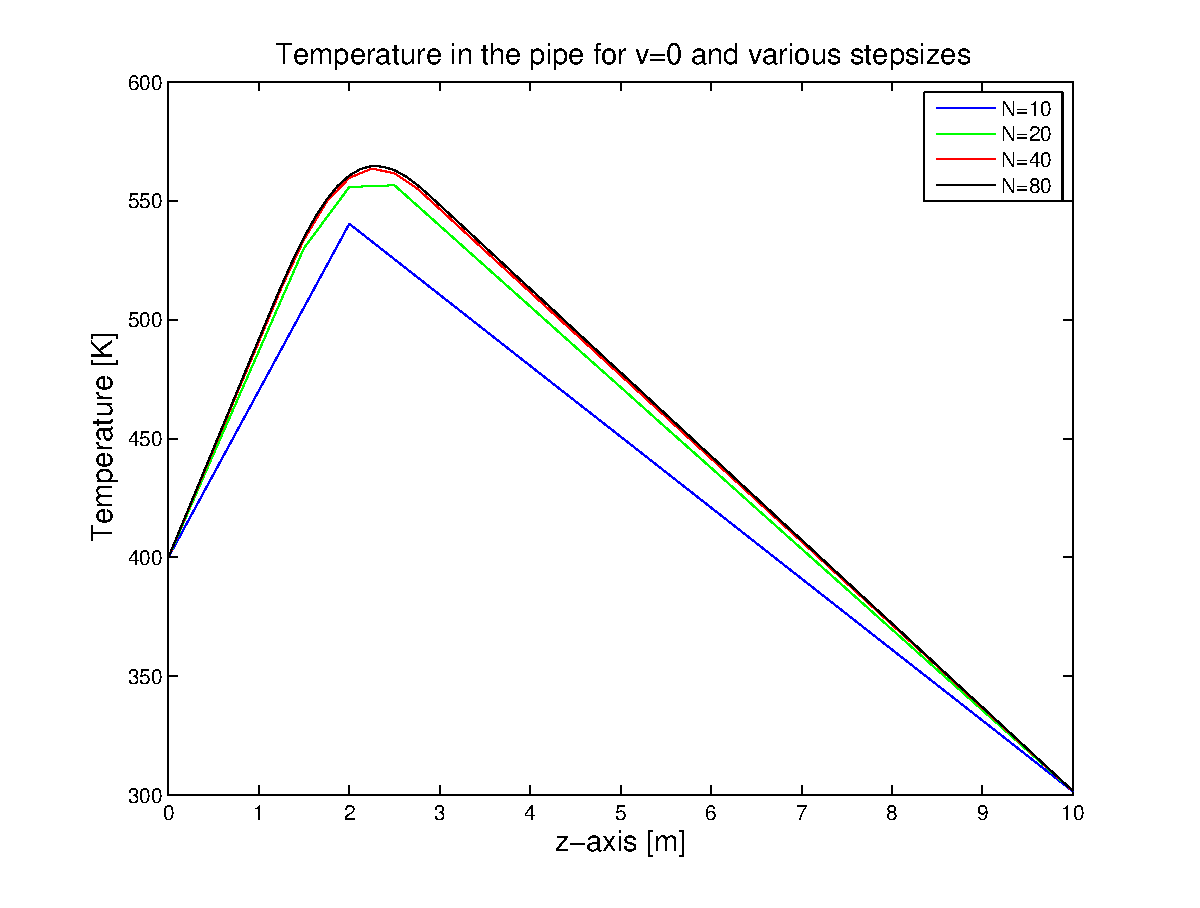
\includegraphics[width = 0.9\textwidth]{./fig1.eps}
\caption{Convergence of solution without convection.}
\label{fig:1}
\end{figure}

We see that increasing $N$ has a great effect on the quality of the solution. It seems to converge towards a smooth curve.

The solution looks like a straight line on the intervals $[0,1]$ and $[3,10]$. This is to be expected. Since $v=0$ and on these intervals the function $Q$ is zero, the equation simplifies to $$\dfrac{d^{2}T}{dz^{2}}=0$$ whose solution is a straight line.

We also check that the convexity is correct. Since $Q$ is non-negative, and again $v=0$, the solution must be concave. Indeed, second derivative is non-positive thanks to the equation.

\subsection*{3) Increasing speed for $N=40$}

Let us set $N=40$. We will now have $v$ vary and take the values $0.1, 0.5, 1,10$. Results on figure~\ref{fig:2}.

\begin{figure}[!h]
\centering
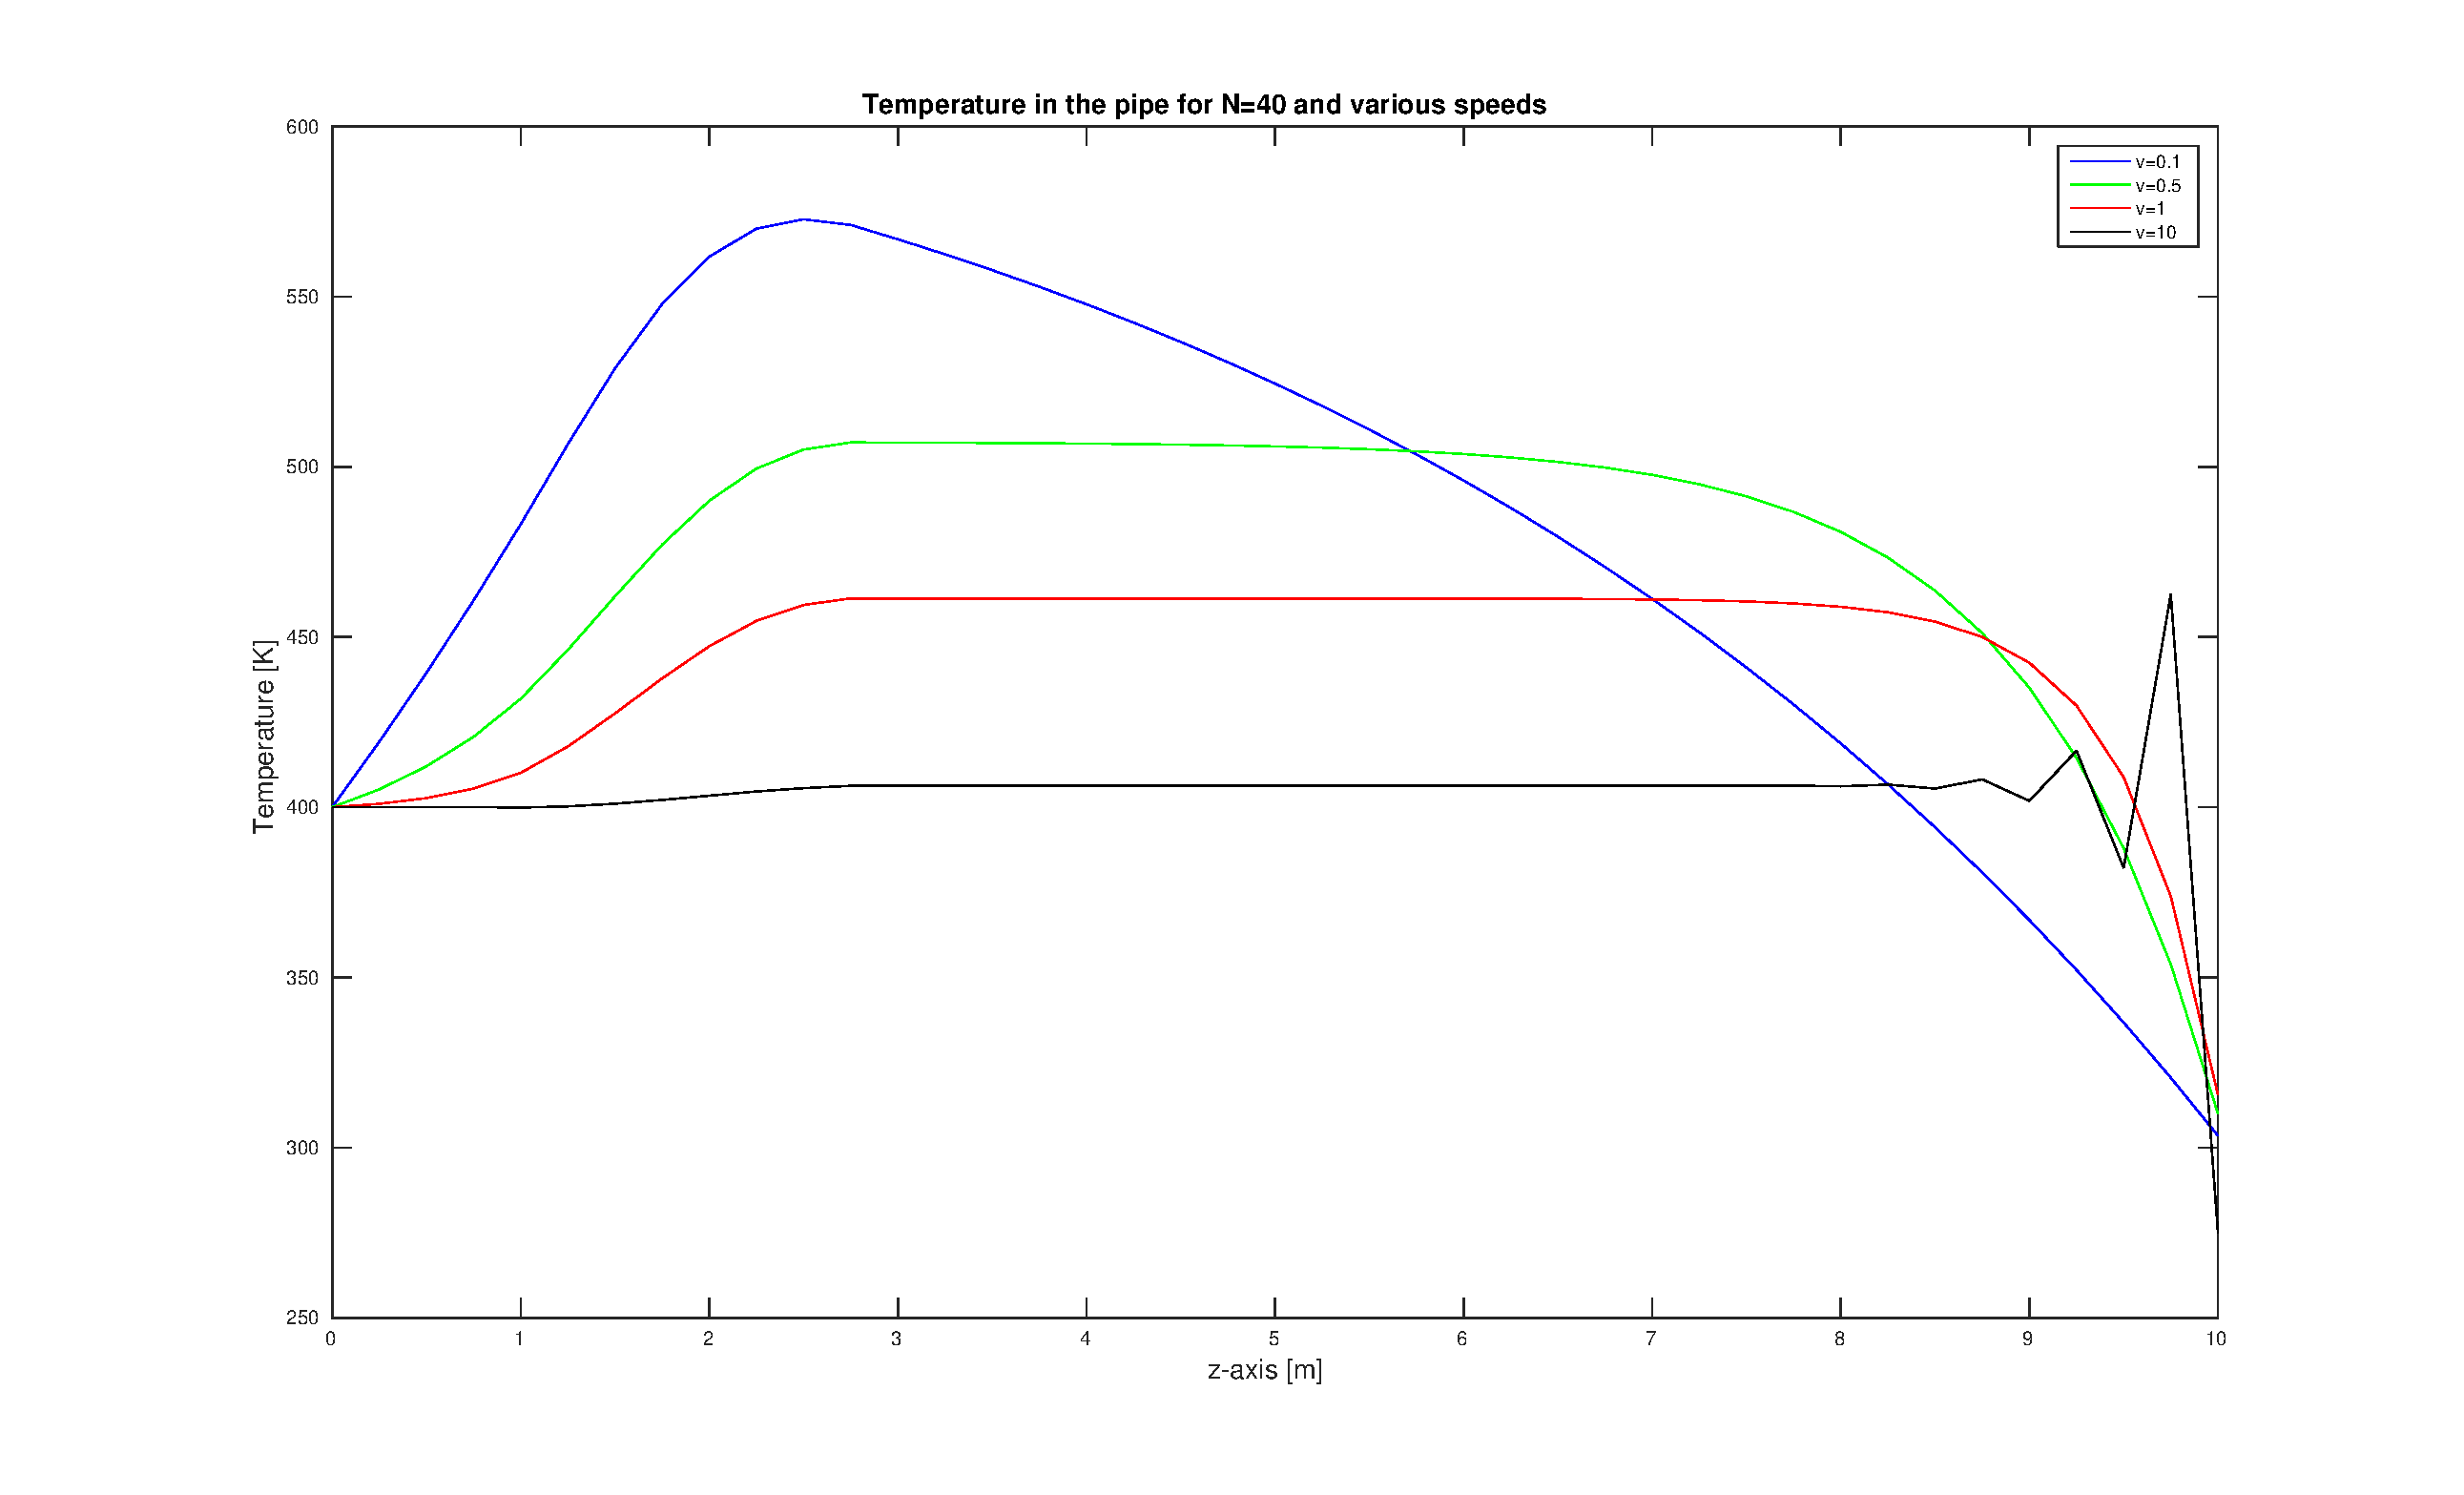
\includegraphics[width = 0.9\textwidth]{./fig2.eps}
\caption{Solution with increasing speed $v$.}
\label{fig:2}
\end{figure}

The maximal temperature decreases as $v$ increases. This makes sense physically since the fluid in the pipe has less time to heat up. For high speeds like $v=10$, the temperature barely changes as the fluid stays a very short time in the pipe.

We clearly notice that oscillations occur when $v=10$. 
The slope of the solution near the end of the rope increases with $v$. This seems to create numerical instabilities for large $v$.

%\subsection{Increasing $N$ for $v=10$}

As we want to see better how the oscillations behave, we now reduce the precision with $N$ for $v$ fixed at 10. Results on figure~\ref{fig:3}.

\begin{figure}[!h]
\centering
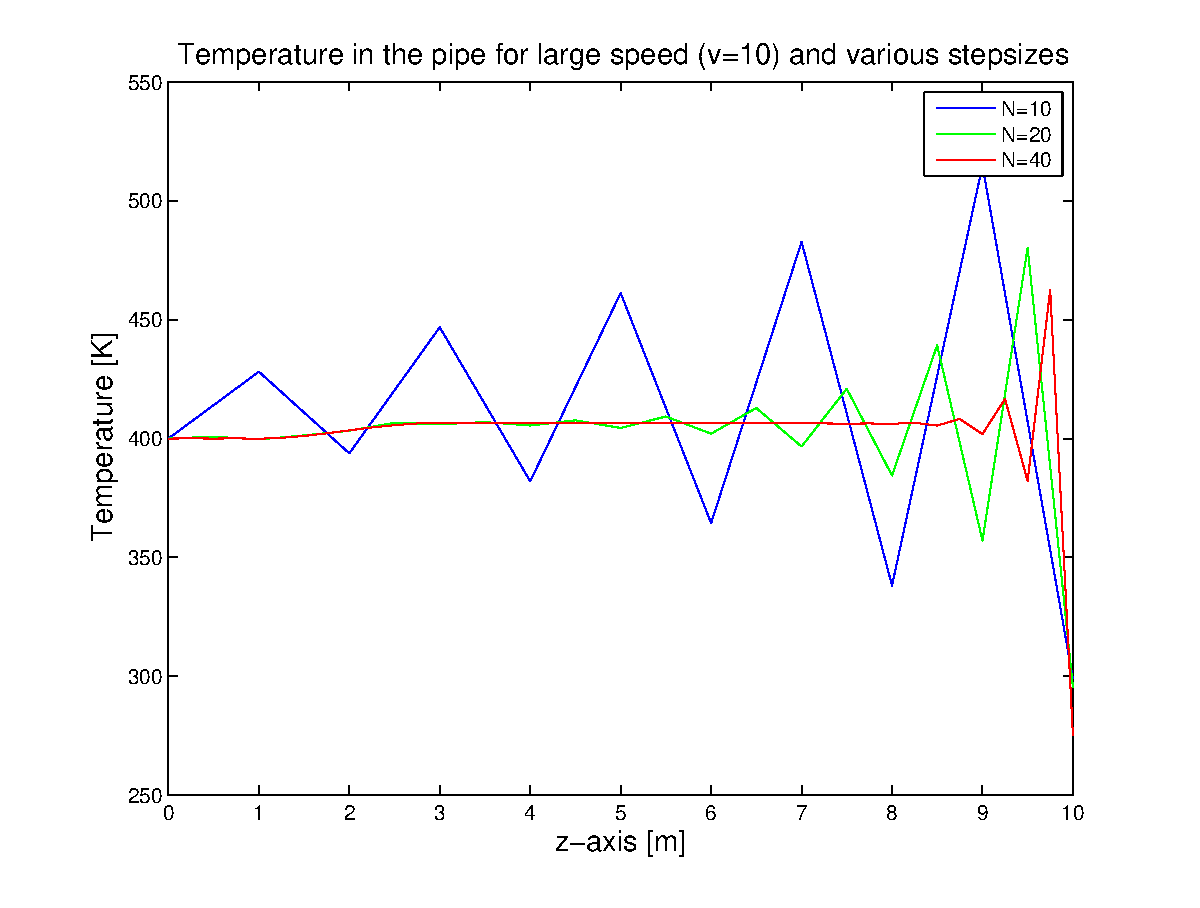
\includegraphics[width = 0.9\textwidth]{./fig3.eps}
\caption{Capture the oscillation with increasing $N$.}
\label{fig:3}
\end{figure}

As the level of the discretization decreases with $N$, we see more and more oscillations. At first ($N=40$) the instabilities are located at the right end of the pipe. As $N$ decreases, the instabilities propagate towards the left end of the pipe.


\end{document}